En el experimento de Millikan se aprecian una serie de fenómenos asociados al 
comportamiento de los fluidos además de la electricidad y magnetismo; en el 
montaje se encuentra una gota de aceite de una densidad $\rho_{ac}$ "("la cual 
está entre dos placas paralelas metálicas gracias a un atomizador")" que se 
encuentra en caída donde alcanza una velocidad terminal $v_c$ gracias a las 
fuerzas de fricción que el aire con densidad $\rho_a$ le ofrece a esta; luego 
se le aplica una diferencia de potencial $V$ a unas placas paralelas de 
distancia $d$ en la región inferior y posterior de la gota teniendo una 
polaridad positiva en la placa superior. En el primer intervalo de tiempo se 
puede realizar un diagrama de cuerpo libre de la gota de aceite.
En la \cref{fig:Montaje} se puede observar el montaje de este experimento.

\begin{figure}[H]                                                               
    \centering                                                                  
    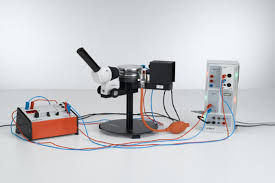
\includegraphics[width=0.35\linewidth]{./images/Montaje-Experimental.jpeg}      
    \caption{Montaje experimental}                                         
    \label{fig:Montaje}                                                         
\end{figure} 

Como se deben medir las posiciones de una gota de agua en un intervalo de 
tiempo, con ayuda de un microscopio se observan las gotas de aceite que se 
encuentran entre las placas. Para medir las posiciones, el lente del
microscopio cuenta con una escala de 20 mm y para medir los tiempos se usa un
cronómetro. En la práctica de laboratorio, se usó una cámara para grabar el 
movimiento de las gotas de aceite, y con ayuda de la línea del tiempo del video
se toman los tiempos.

Como se realizaron videos para medir las posiciones de las gotas de aceite, se 
utilizó el software de Tracker Video, programa en el cual, al ajustar una
escala se puede obtener la posicion del objeto seleccionado, en este caso las 
gotas, frame por frame del video. Una vez que se hace toman los datos con 
Tracker, estos se pueden exportar en arhivos para posteriormente hacer el 
análisis de los mismos. En la \cref{fig:Tracker} se puede observar la interfaz
del software.

\begin{figure}[H]
    \centering
    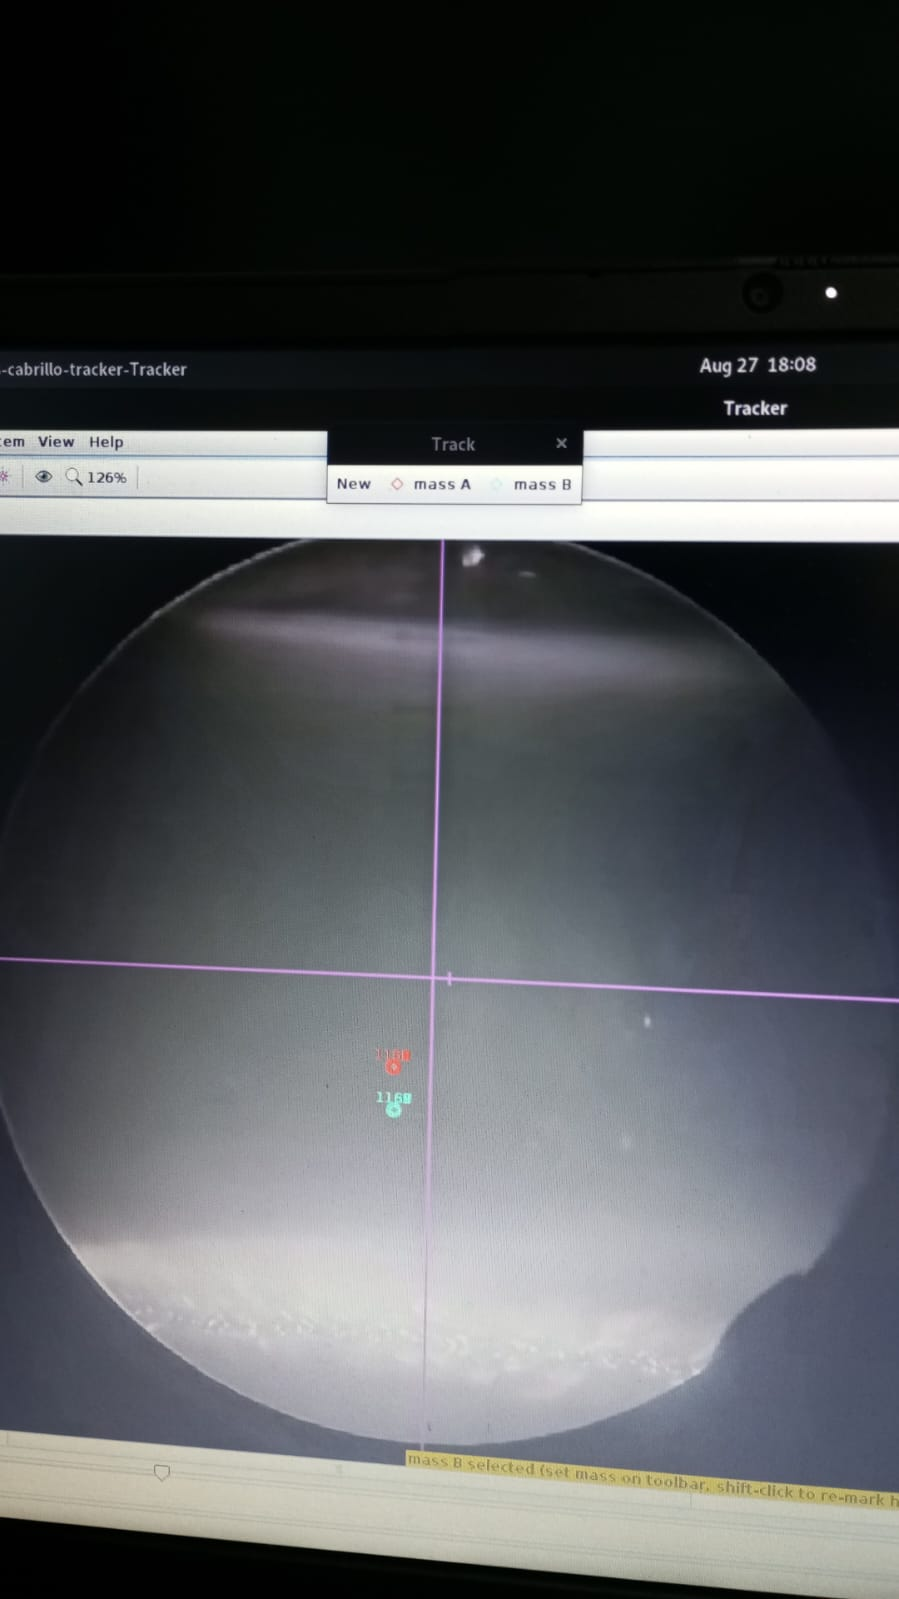
\includegraphics[width=0.35\linewidth]{./images/Interfaz-Tracker.jpeg}
    \caption{Interfaz de Tracker Video}
    \label{fig:Tracker}
\end{figure}
